\section{Etapa de diseño}
Lo primero que se diseñó para este proyecto fue la nueva base de datos. Ya se tenía un gran avance para esta etapa, pues se tomó como base la base de datos original, sólo se realizaron algunos ajustes y se crearon nuevas tablas para bitácoras.

Posteriormente, el proyecto se decidió dividir en 2 desarrollos: uno para Frontend y el otro para Backend. Con esto también se decidieron las tecnologías que se utilizarían para los desarrollos y las actividades que estos conllevarían:
    \begin{itemize}
        \item Para el Frontend se utilizó Next.js.
        \item Para el Backend se utilizó Node.js con Express.js.
        \item Para los servicios en la nube se utilizó AWS.\@
    \end{itemize}

La estructura de cada proyecto dependía del framework con el que se trabajara y de la decisión del desarrollador. Next.js es un framework opinionado, por lo que ya proporciona reglas para la estructura del proyecto (Ver Figura 50); en cambio, Express.js es un framework no opinionado por lo que se decidió una estructura del proyecto.

    \begin{figure}[H]
        \begin{center}
            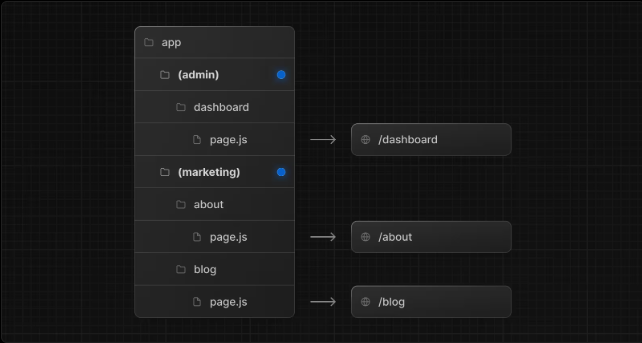
\includegraphics[scale=0.60]{img/resultados/nextjs-structure.png}
            \caption{Estructura de un proyecto en Next.js.}
            \label{fig:nextjs-estructura}
        \end{center}
    \end{figure}

La carpeta raíz lleva por nombre ``src'', y dentro de esta existen 3 carpetas:
    \begin{itemize}
        \item ``configurations'': Dentro de esta carpeta se guardan archivos de configuración para diferentes herramientas que se usan en el poryecto como CORS o las conexiones a las bases de datos.
        \item ``data'': En esta carpeta se guardan los archivos que contienen las consultas que se realizan para manipular la base de datos.
        \item ``server'': Aquí se guardan archivos que permiten interactuar directamente con el servidor de Express.js, por ejemplo, controladores, servicios, rutas, middlewares, estre otros.
    \end{itemize}

Por último, el diseño de las interfaces ya se tenía resuelto pues para el Frontend se utilizó una plantilla llamada ``DashTail''. Esta plantilla proporciona diversas páginas y componentes que pueden ser manipulados para adaptarlos a las necesidades del proyecto.